%TODO no numeri a lato del codice
\begin{frame}[t,plain]
\titlepage
\end{frame}

\begin{frame}{Steps}
	\begin{itemize}
		\item Calibration
		\item Unwrapping
		\item Detection
	\end{itemize}
\end{frame}


\begin{frame}{Calibration}
	Given a set of pictures taken with a camera, the object of this step is to find the camera matrix $A$ and the distortion coefficients $\dot{d}$.\newline
	\vfill
	\[
		A=\begin{bmatrix}
			f_x&0&c_x\\
			0&f_y&c_y\\
			0&0&1\\
		\end{bmatrix}\qquad
		\begin{matrix}
			x_{distorted}=x\left(1+k_1r^2+k_2r^4+k_3r^6\right)\\
			y_{distorted}=y\left(1+k_1r^2+k_2r^4+k_3r^6\right)\\
			x_{distorted}=x+\left[2p_1xy+p_2\left(r^2+2x^2\right)\right]\\
			y_{distorted}=y+\left[p_1\left(r^2+2y^2\right)+2p_2xy\right]\\
			\dot{d}=(k_1, k_2, p_1, p_2, k_3)
		\end{matrix}
	\]
	\vfill
\end{frame}


\begin{frame}{Calibration}
	\begin{figure}[H]
		\begin{minipage}{0.48\linewidth}
			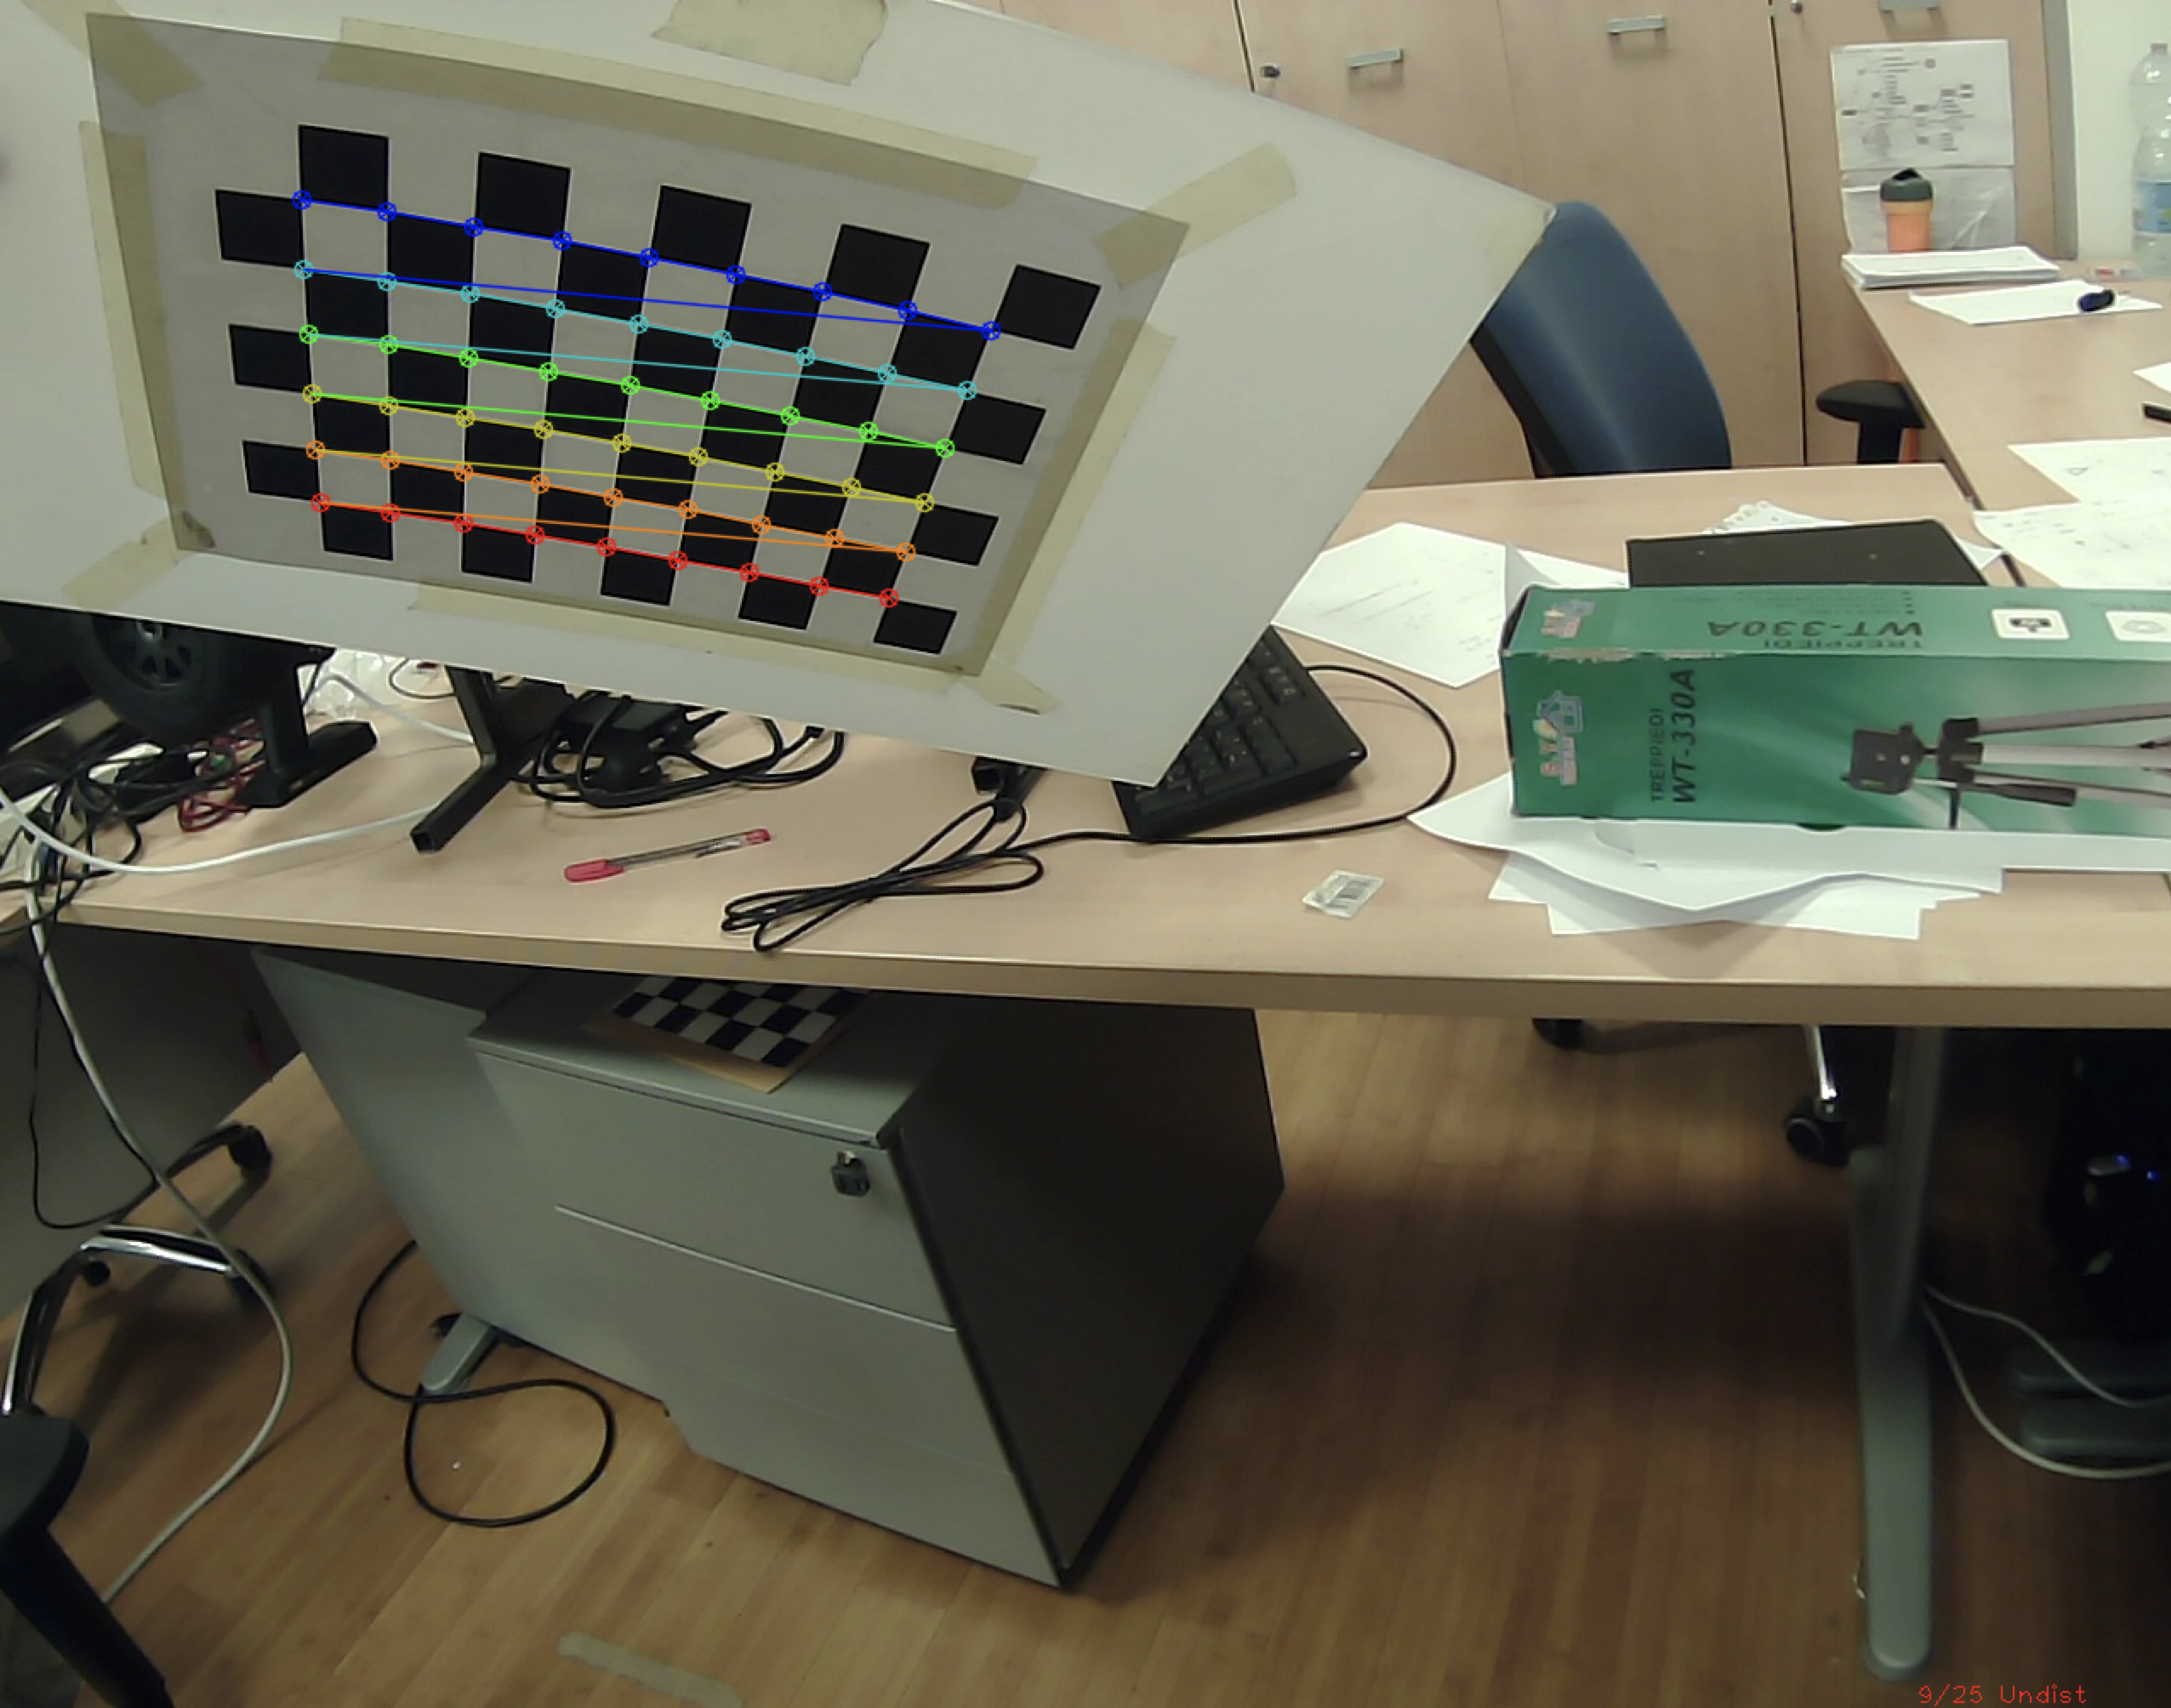
\includegraphics[width=\linewidth]{Immagini/Chessboard1}
		\end{minipage}
		\vspace{0.04\linewidth}
		\begin{minipage}{0.48\linewidth}
			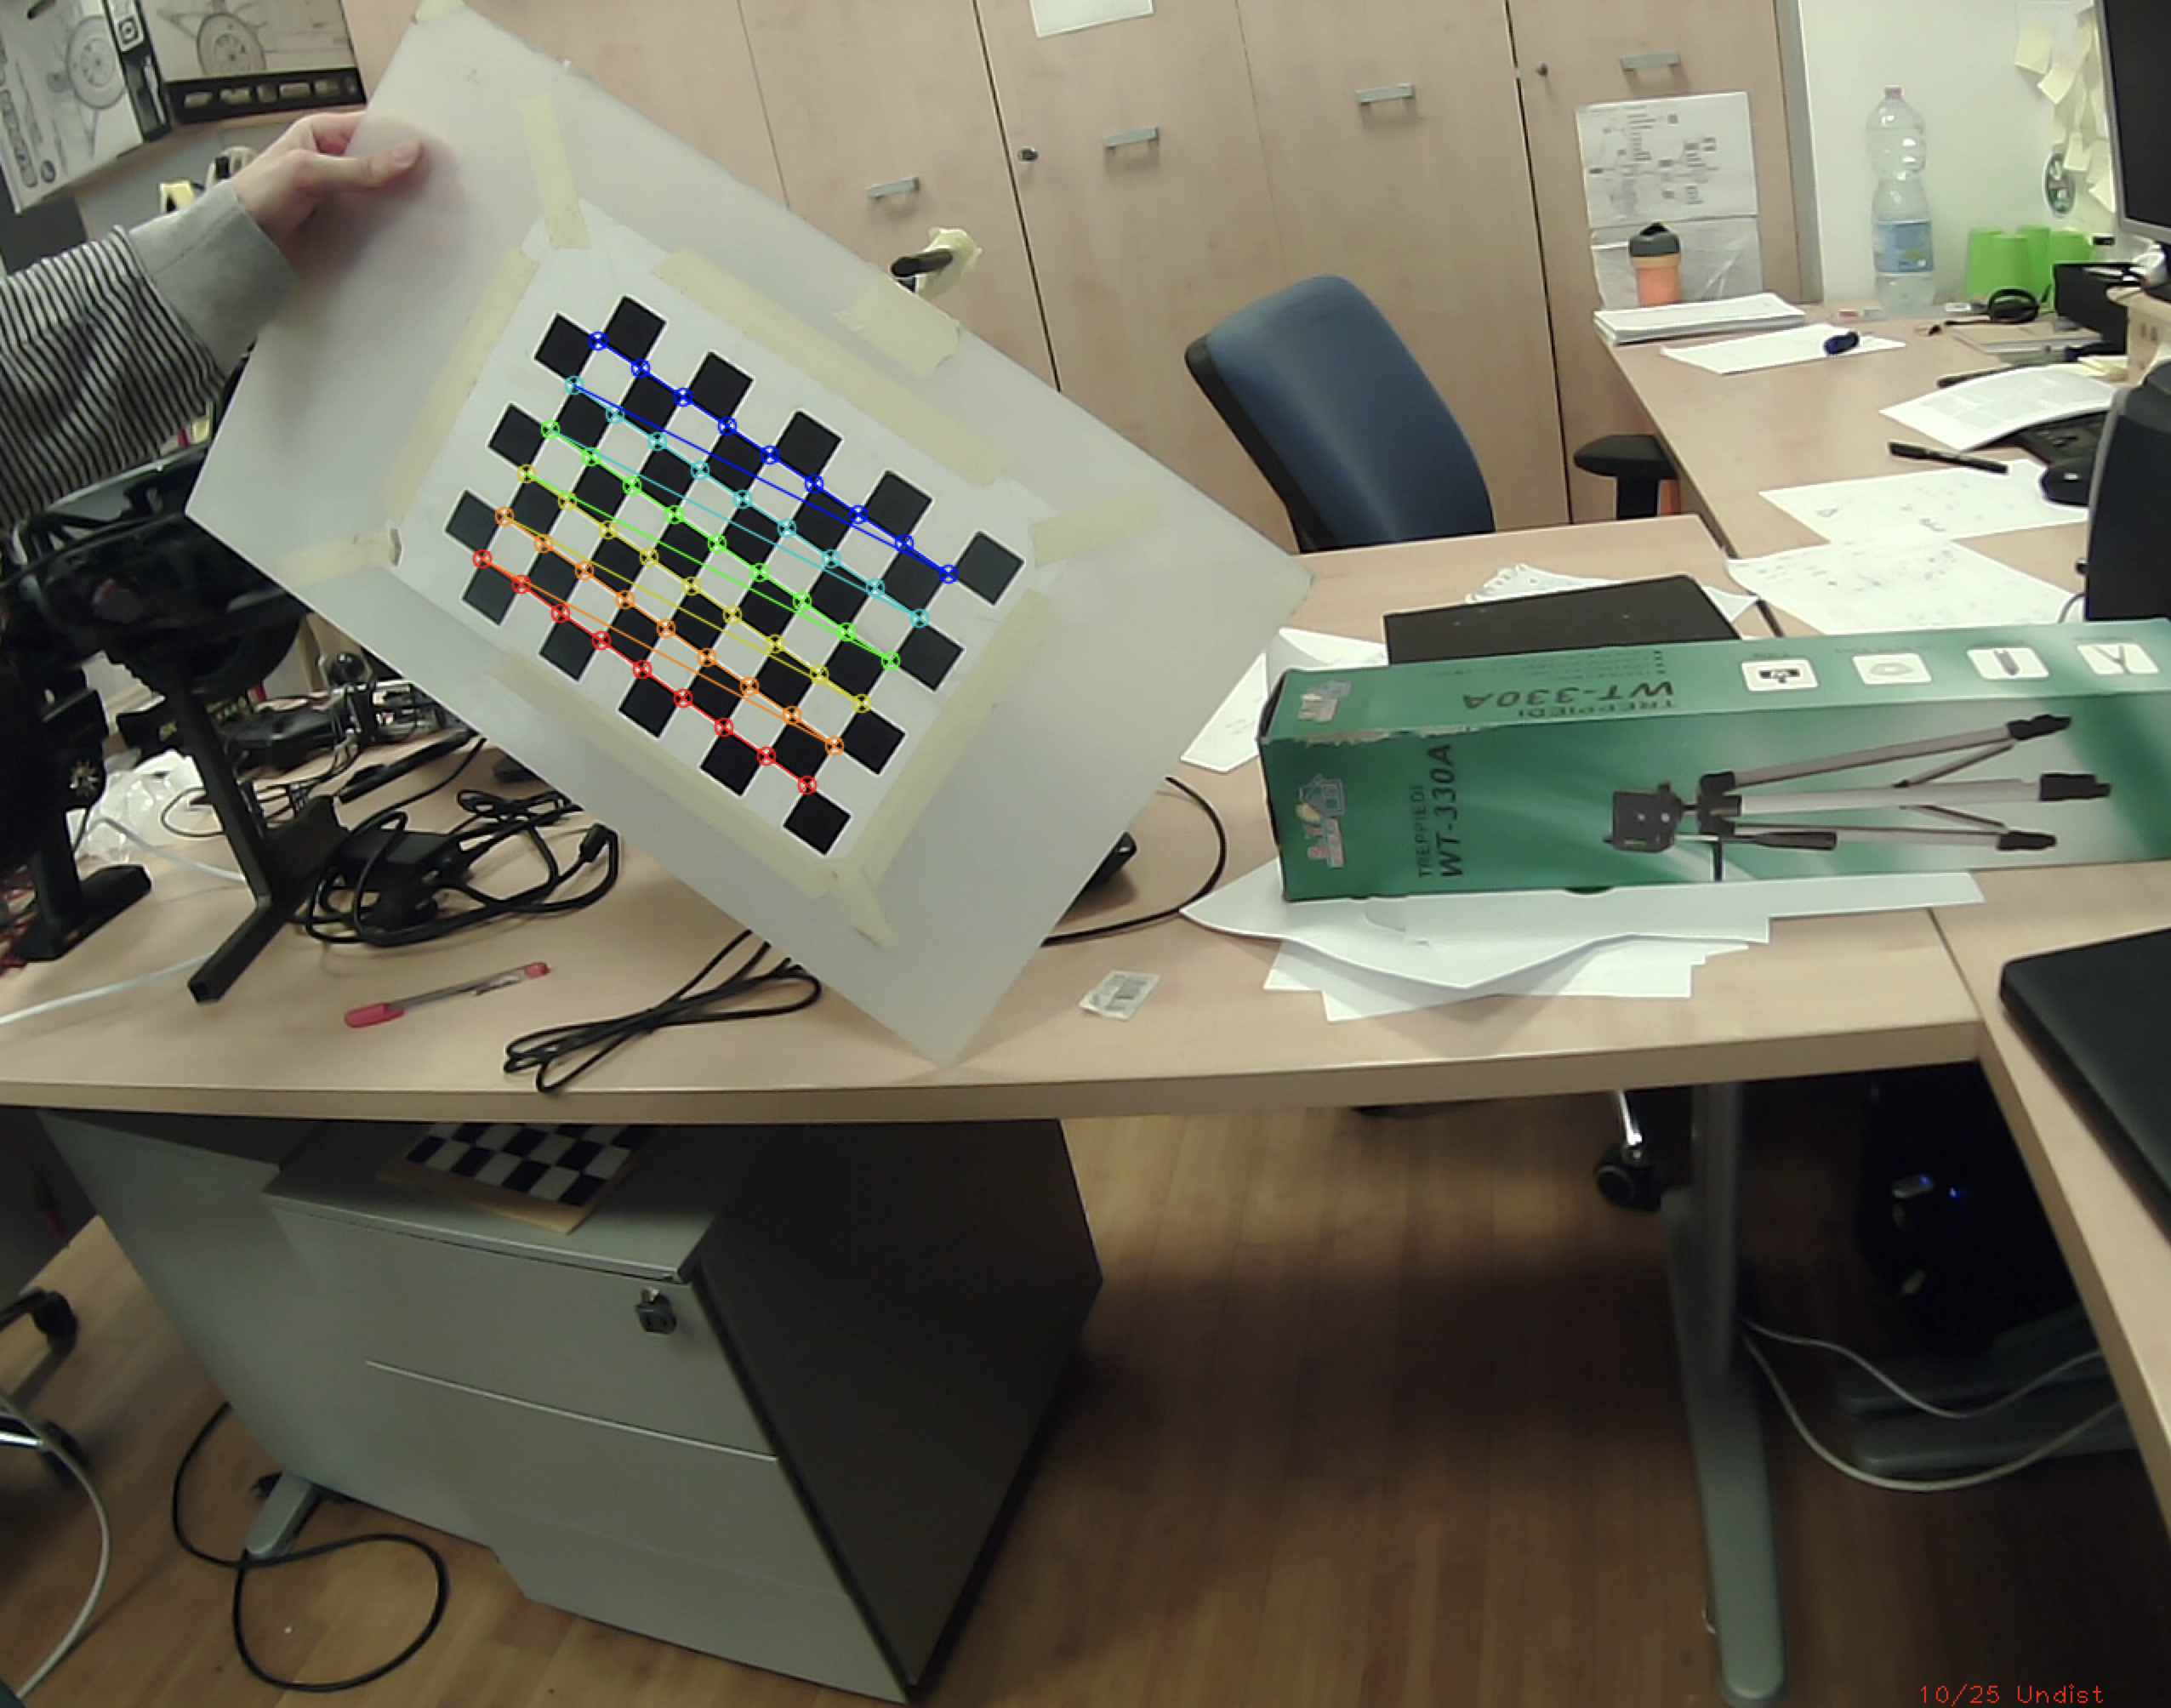
\includegraphics[width=\linewidth]{Immagini/Chessboard2}
		\end{minipage}
	\end{figure}
\end{frame}


\begin{frame}{Calibration}
	\begin{figure}[H]
		\begin{minipage}{0.48\linewidth}
			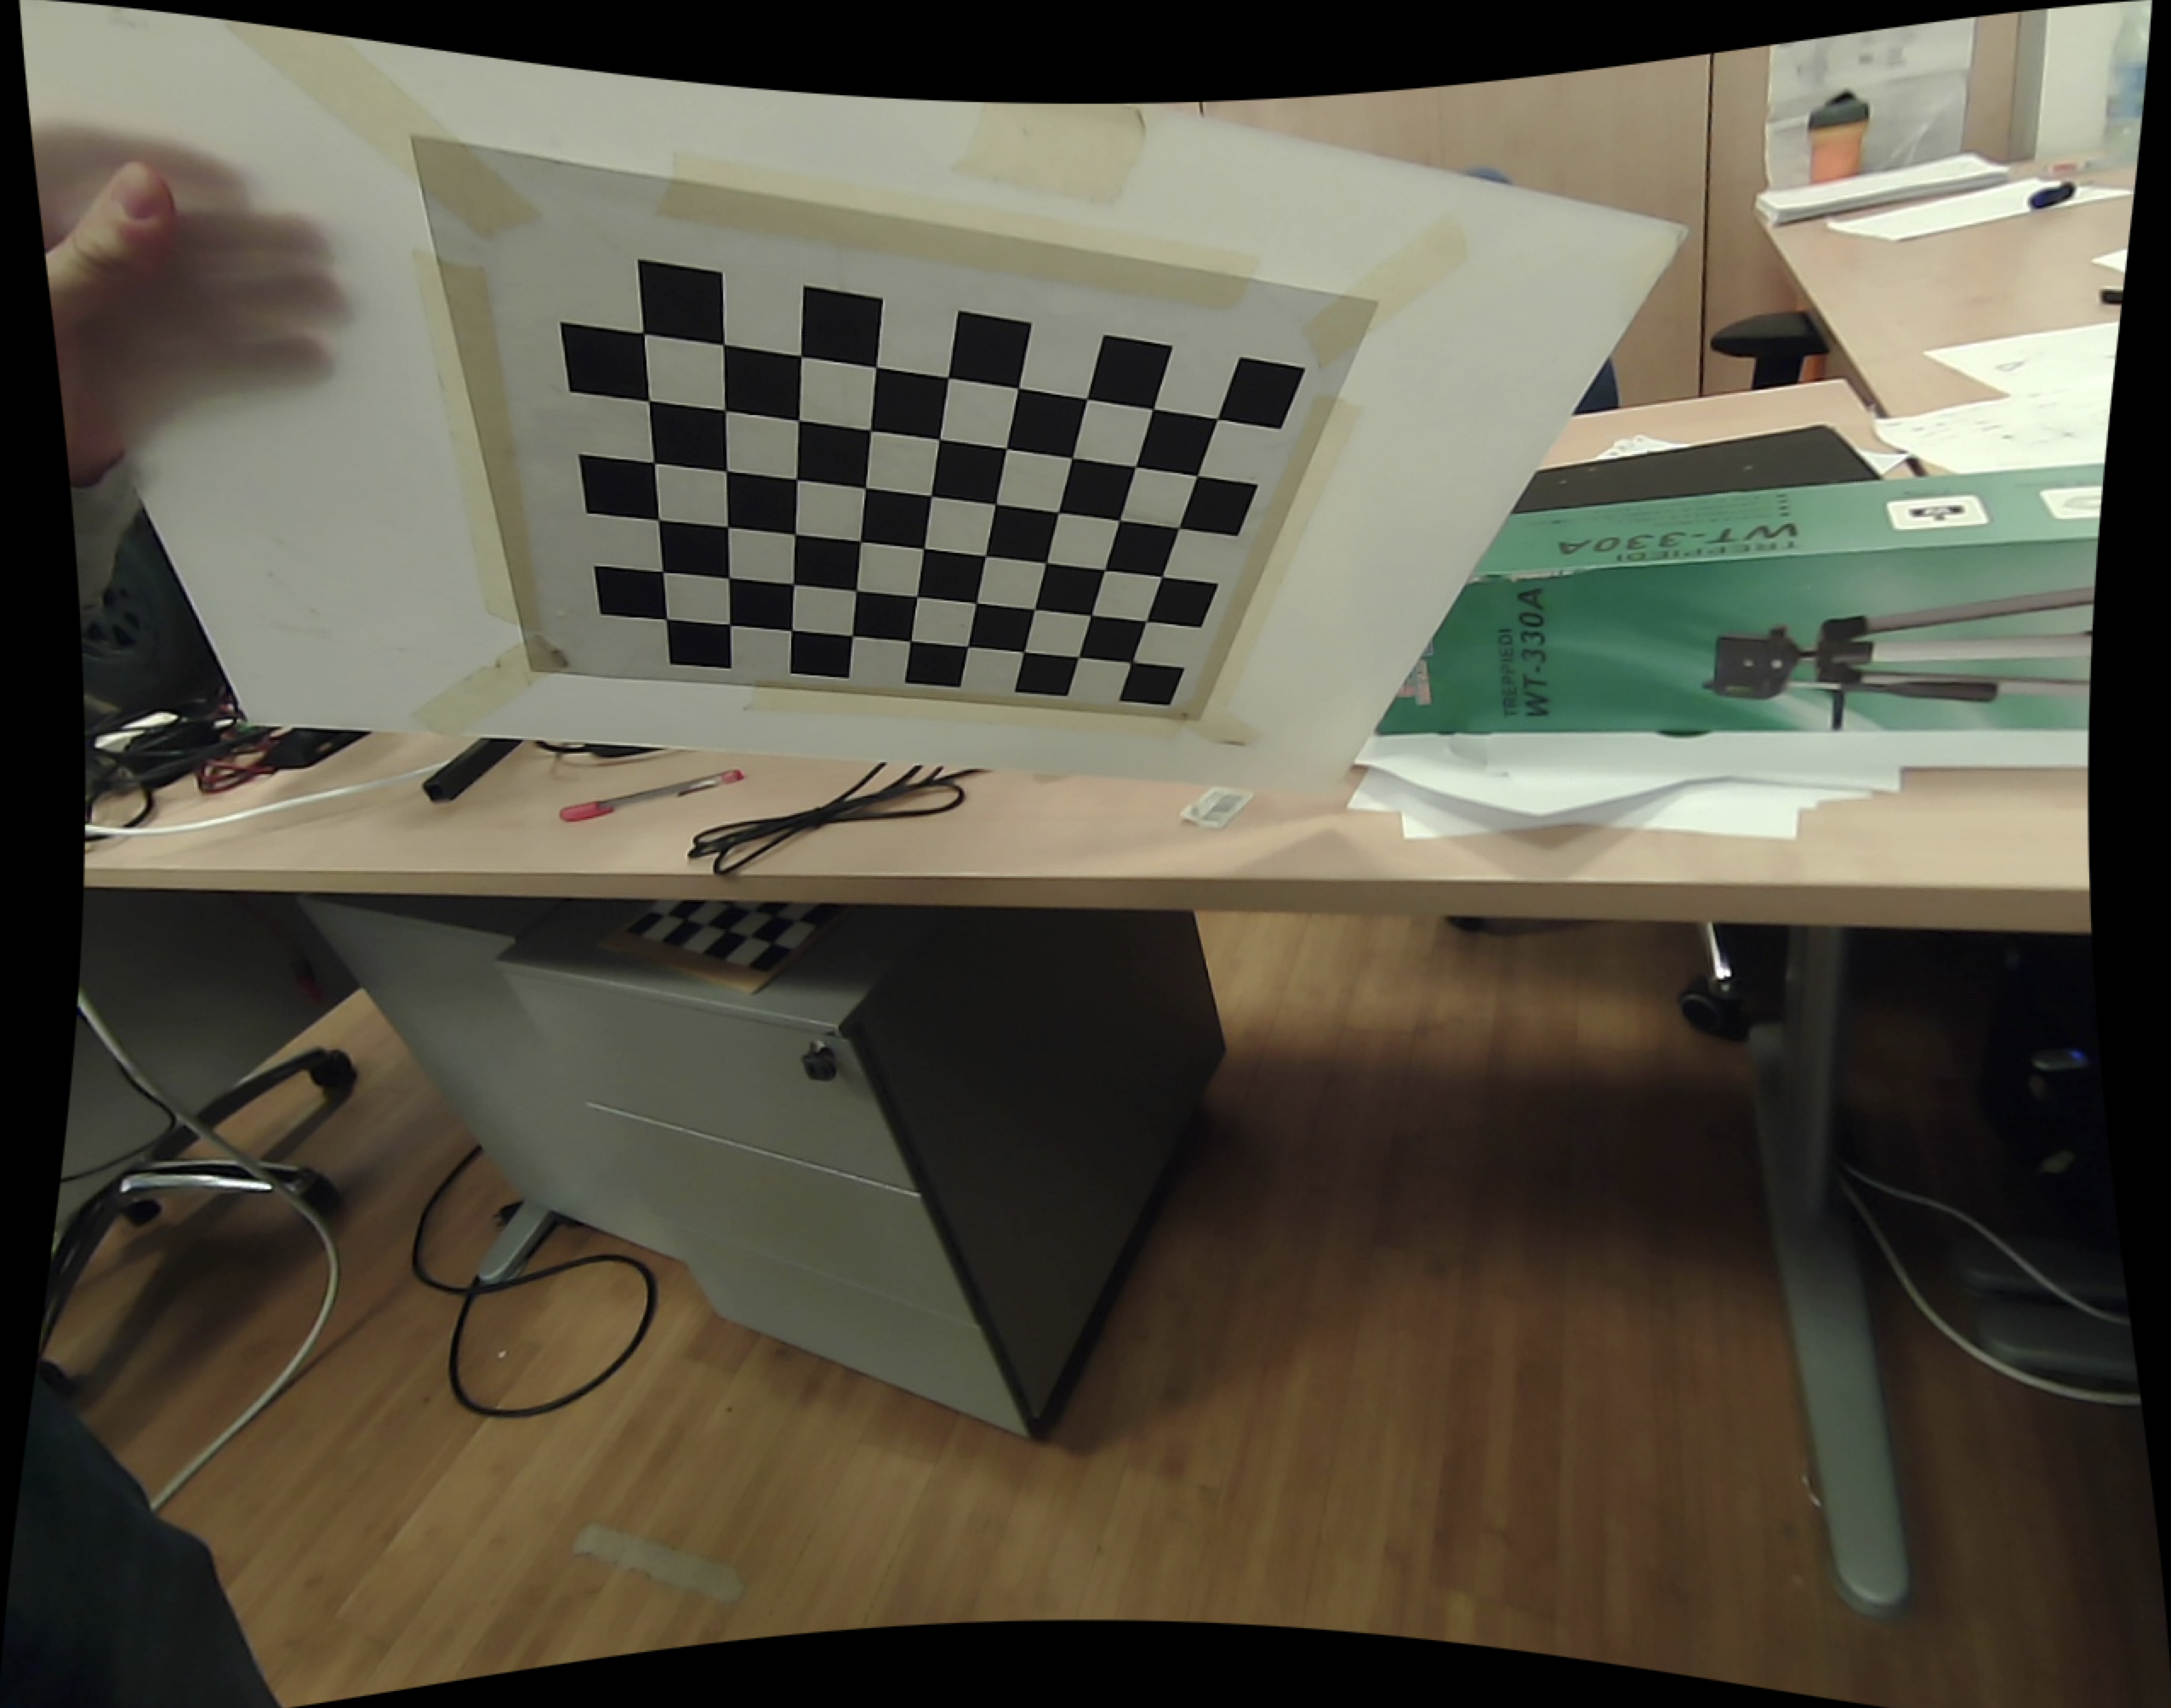
\includegraphics[width=\linewidth]{Immagini/Chessboard1Calibrated}
		\end{minipage}
		\vspace{0.04\linewidth}
		\begin{minipage}{0.48\linewidth}
			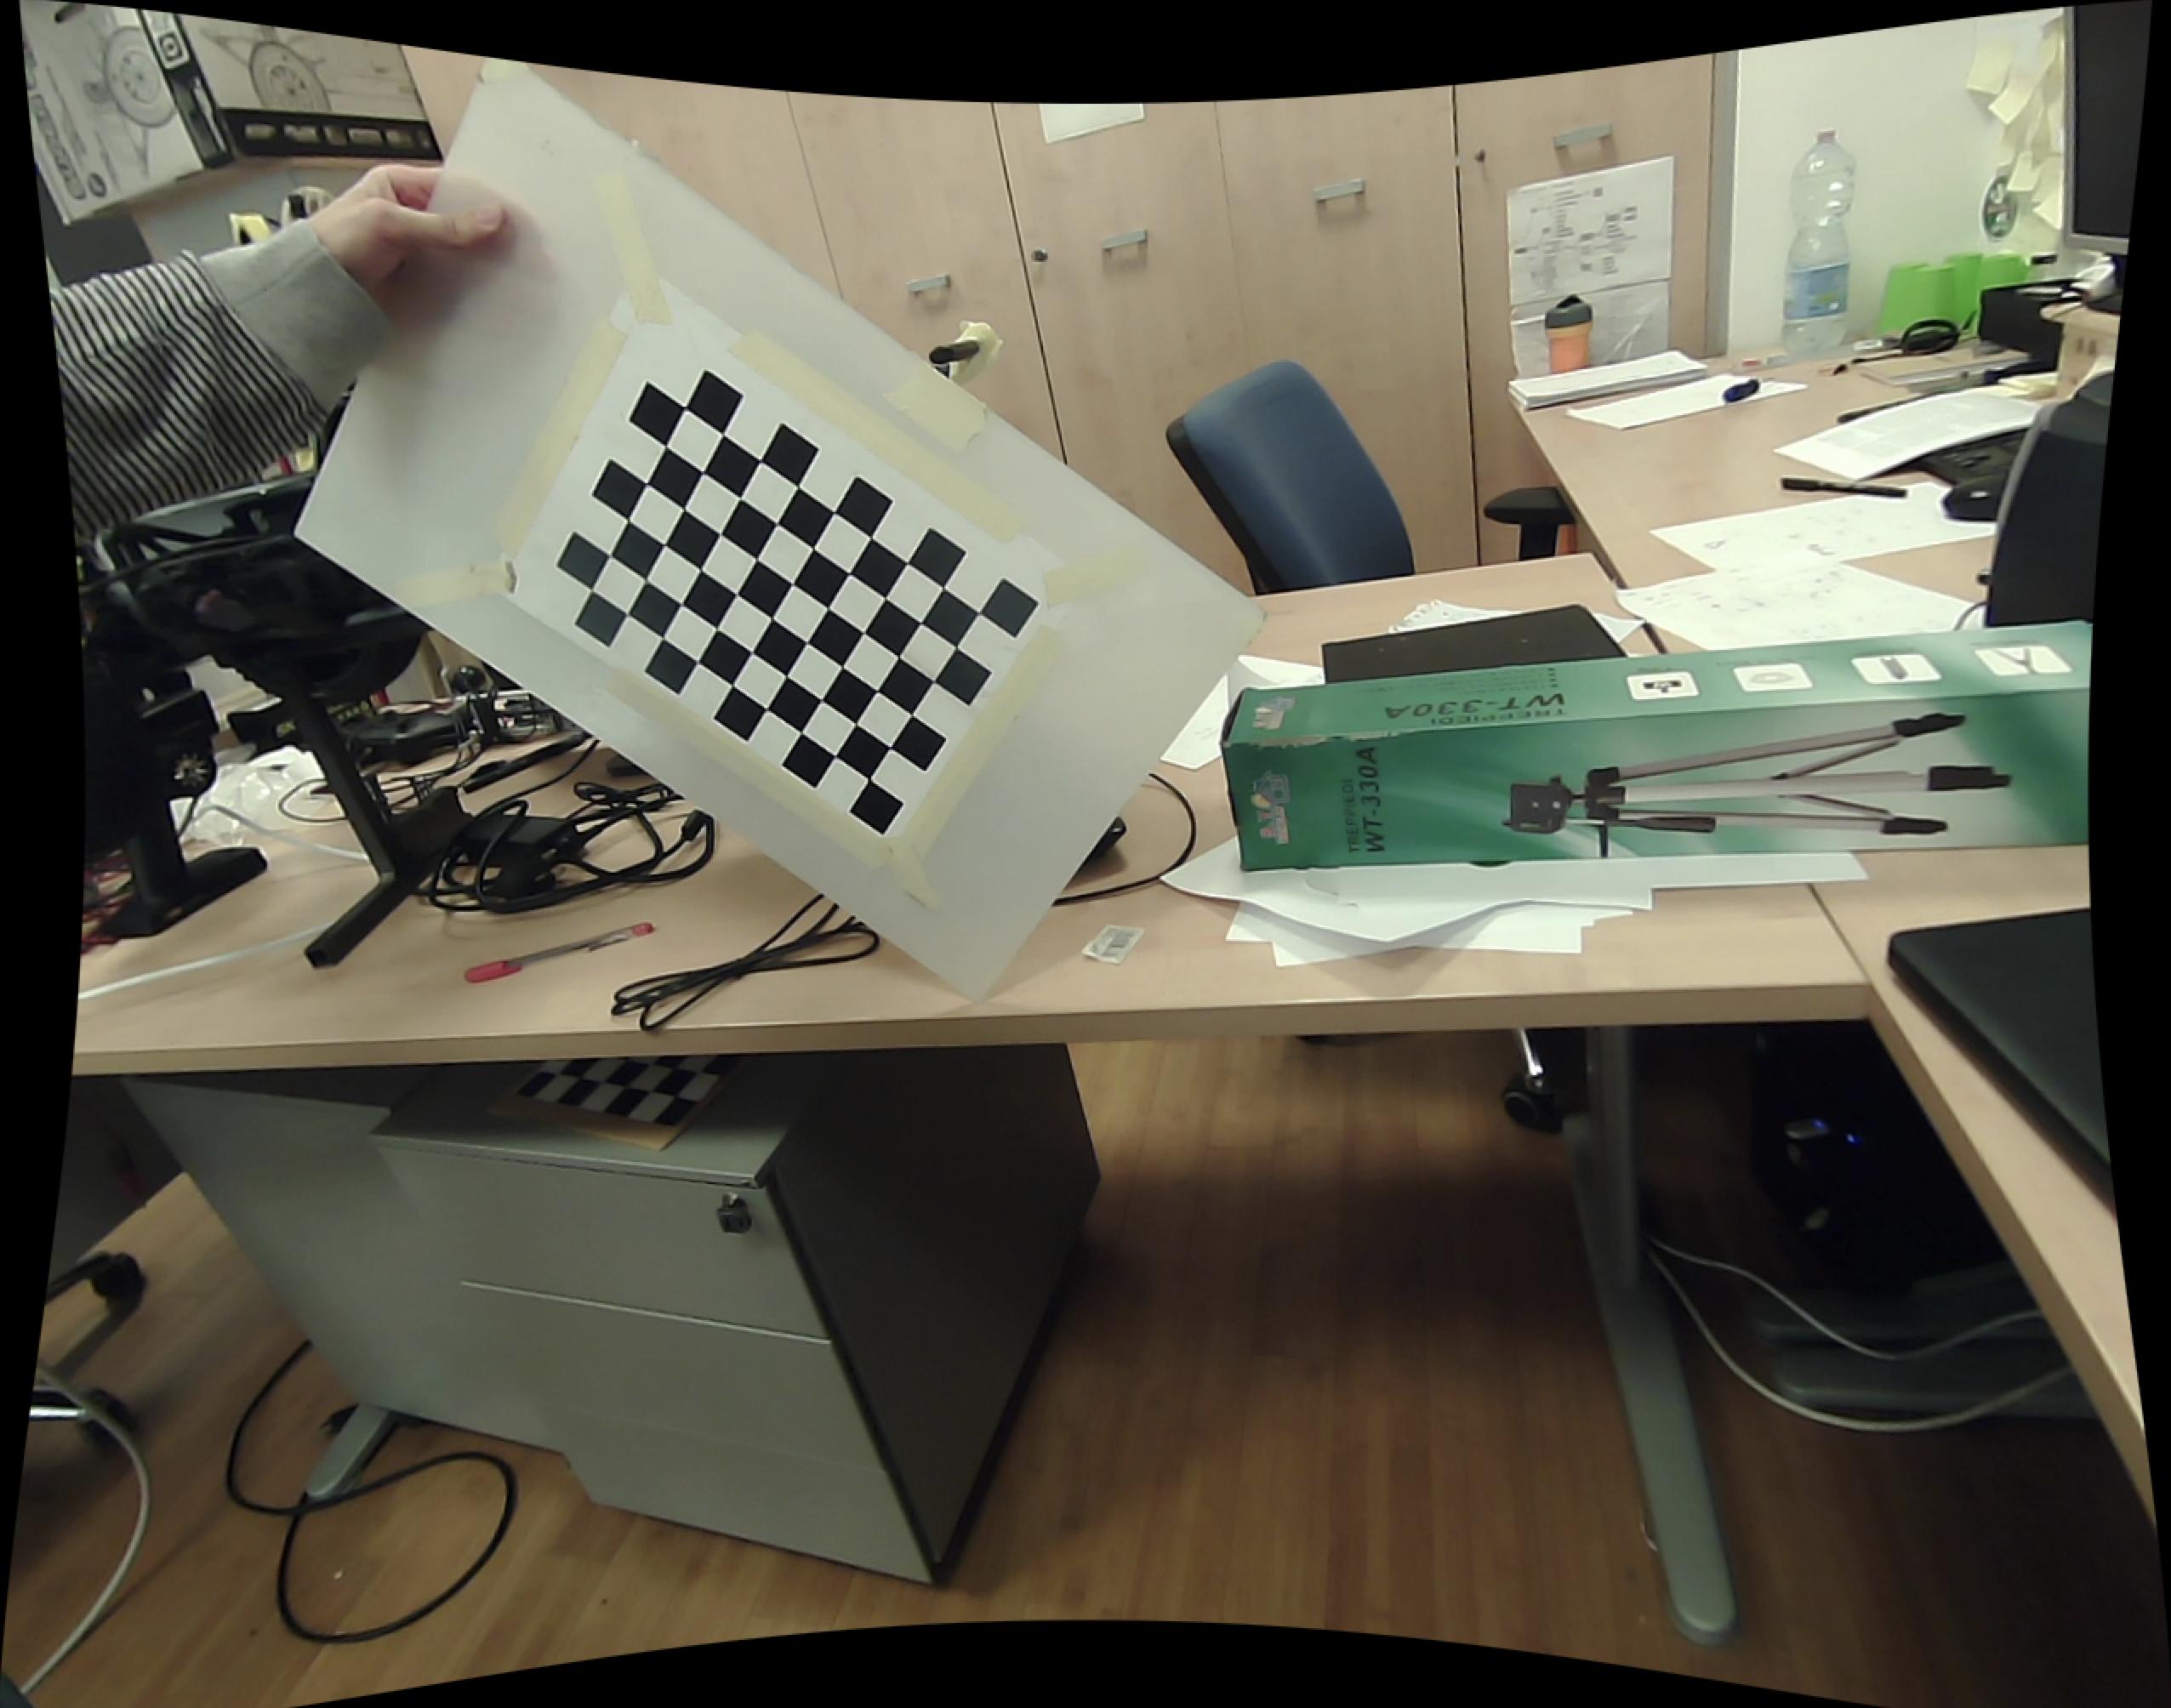
\includegraphics[width=\linewidth]{Immagini/Chessboard2Calibrated}
		\end{minipage}
	\end{figure}
	\stsize
	\[A=\begin{bmatrix}
		8.4247565095622963\times10^2 & 0 & 6.3709750745251142\times10^2\\
		0 & 8.4247565095622963\times10^2 & 4.9404840840221556\times10^2\\
		0 & 0 & 1
	\end{bmatrix}\]\[
	\dot{d}=(-2.5214446354851400\times10^{-1}, 7.2467634259951161\times10^{-2},\]\[-3.7212601356153754\times10^{-3}, 4.3313659139950872\times10^{-4}, 0)
	\]
\end{frame}

\begin{frame}{Unwrapping}
	
\end{frame}











